\documentclass[11pt]{article}

\usepackage{tabularx}
\usepackage[margin=1in]{geometry}
\usepackage{amsmath, amssymb, amsthm}
\usepackage{graphicx}
\usepackage{booktabs}
\usepackage{tabularx}
\usepackage{listings}
\usepackage{xcolor}
\usepackage{hyperref}
\usepackage{enumitem}
\usepackage{seqsplit}
\usepackage{parskip}
\usepackage{float}

\hypersetup{
  colorlinks=true,
  linkcolor=blue,
  urlcolor=blue,
  citecolor=blue
}

% ------- Styling for problems and answers -------
\newcommand{\problem}[2]{%
  \vspace{0.6em}%
  \noindent\textbf{Problem (\texttt{#1})}\hfill\textit{#2 points}\par%
  \vspace{0.2em}\hrule\vspace{0.4em}%
}
\newcommand{\subq}[1]{\vspace{0.3em}\noindent\textbf{(#1)}\ }
\newcommand{\deliverable}[1]{\vspace{0.2em}\noindent\textit{Deliverable:} #1\par}

% Answer block: swap this for your own preferred style
\newenvironment{answer}{%
  \vspace{0.3em}%
  \noindent\textbf{Answer.}\begin{quote}%
}{%
  \end{quote}\vspace{0.4em}%
}

\lstset{
  basicstyle=\ttfamily\small,
  breaklines=true,
  frame=single,
  columns=fullflexible,
}

\graphicspath{{figures/}}

\title{CS336 Assignment 2: Systems --- Writeup}
\author{James Liu}
\date{\today}

\begin{document}
\maketitle

\tableofcontents
\vspace{1em}

% =========================================================
\section{Profiling and Benchmarking}
% =========================================================

\problem{benchmarking\_script}{4}

\subq{a} Write a script to perform basic end-to-end benchmarking of the forward pass, backward pass, and optimizer step in your model (given hyperparameters, random batch, warm-up steps, timed steps for forward / forward+backward / full training step, with \texttt{torch.cuda.synchronize()} after each step).
\deliverable{A script that initializes a basics Transformer with given hyperparameters, creates a random batch, and times forward-only, forward-and-backward, and full training steps.}
\begin{answer}
See $cs336\_systems/benchmarking.py$
\end{answer}

\newpage
\subq{b} Time the forward, backward, and optimizer step for each model size in Table~1 using 5 warmup steps and 10 measurement steps. How long does a forward pass take? A backward pass? Is variability / std small?
\deliverable{A 1--2 sentence response with your timings.}
\begin{answer}
  \begin{table}[H]
    \centering
    \caption{Benchmark results across model sizes (5 warm up steps, 10 training steps).}
    \label{tab:model-benchmark-results}
    \begin{tabular}{llll}
    \toprule
    Size & forward & forward-back & forward-back-optimizer \\
    \midrule
    small & 0.0165 ± 0.0000 & 0.0488 ± 0.0000 & 0.0561 ± 0.0000 \\
    med & 0.0472 ± 0.0001 & 0.1398 ± 0.0007 & 0.1566 ± 0.0011 \\
    large & 0.1063 ± 0.0000 & 0.3168 ± 0.0069 & 0.3447 ± 0.0009 \\
    xl & 0.2935 ± 0.0004 & 0.8636 ± 0.0005 & 0.9453 ± 0.0001 \\
    10b & 0.9448 ± 0.0002 & 2.8113 ± 0.0006 & OOM \\
    \bottomrule
    \end{tabular}
    \end{table}  
    See table for timing of forward, forward-backward, and forward-backward-optimizer steps. 
    The forward-only, forward+backward, and full training-step timings are shown in 
    Table~\ref{tab:model-benchmark-results}. Forward+backward is roughly 3x 
    slower than forward-only due to gradient computation, and adding the optimizer 
    step introduces a smaller additional cost. The standard deviations are extremely 
    small after warmup, which shows that the GPU runs are extremely consistent. 
\end{answer}

\subq{c} Repeat the analysis without warmup, and with 1 or 2 warmup steps. How do results change? Why?
\deliverable{A 2--3 sentence response.}
\begin{answer}
  \begin{table}[H]
    \centering
    \caption{Benchmark results across model sizes (no warm up steps, 10 training steps).}
    \label{tab:model-benchmark-results-no-warmup}
    \begin{tabular}{llll}
    \toprule
    Size & forward & forward-back & forward-back-optimizer \\
    \midrule
    small & 0.0555 ± 0.1168 & 0.1181 ± 0.2001 & 0.1161 ± 0.1653 \\
    med & 0.0817 ± 0.1043 & 0.2044 ± 0.1923 & 0.2330 ± 0.2127 \\
    large & 0.1070 ± 0.0024 & 0.3605 ± 0.1424 & 0.3610 ± 0.0468 \\
    xl & 0.3300 ± 0.1033 & 0.8694 ± 0.0265 & 1.0079 ± 0.1902 \\
    10b & 0.9624 ± 0.0501 & 2.8153 ± 0.0015 & OOM \\
    \bottomrule
    \end{tabular}
    \end{table}    

    As seen above in the table, without warming up the GPU beforehand, each of the computations take significantly longer (since now there is the overhead for warming up the GPU--compiling the kernels, allocating memory, etc...)

  \begin{table}[H]
    \centering
    \caption{Benchmark results across model sizes (one warm up step and 10 training steps).}
    \label{tab:model-benchmark-results-one-warmup-step}
    \begin{tabular}{llll}
    \toprule
    Size & forward & forward-back & forward-back-optimizer \\
    \midrule
    small & 0.0164 ± 0.0000 & 0.0483 ± 0.0002 & 0.0634 ± 0.0187 \\
    med & 0.0469 ± 0.0001 & 0.1390 ± 0.0000 & 0.1586 ± 0.0032 \\
    large & 0.1062 ± 0.0001 & 0.3135 ± 0.0001 & 0.3496 ± 0.0222 \\
    xl & 0.2927 ± 0.0003 & 0.8640 ± 0.0005 & 0.9422 ± 0.0004 \\
    10b & 0.9451 ± 0.0008 & 2.8198 ± 0.0001 & OOM \\
    \bottomrule
    \end{tabular}
    \end{table}
      

  \begin{table}[H]
    \centering
    \caption{Benchmark results across model sizes (2 warm up steps and 10 training steps).}
    \label{tab:model-benchmark-results-two-warmups}
    \begin{tabular}{llll}
    \toprule
    Size & forward & forward-back & forward-back-optimizer \\
    \midrule
    small & 0.0165 ± 0.0000 & 0.0489 ± 0.0000 & 0.0569 ± 0.0006 \\
    med & 0.0471 ± 0.0000 & 0.1396 ± 0.0001 & 0.1573 ± 0.0003 \\
    large & 0.1064 ± 0.0005 & 0.3185 ± 0.0105 & 0.3443 ± 0.0007 \\
    xl & 0.2927 ± 0.0003 & 0.8641 ± 0.0006 & 0.9453 ± 0.0009 \\
    10b & 0.9452 ± 0.0003 & 2.8204 ± 0.0010 & OOM \\
    \bottomrule
    \end{tabular}
    \end{table}      

    As seen in the above table comapred to the one without warm up steps, just warming up the GPU for one iteration greatly reduces the total training time. The result between 1 or 2 warm up steps is much closer to the 10 warm up steps one since most of the overhead (e.g. CUDA context initialization, allocator warm up, etc...) is eliminated if we just do one warm up step ahead of timing the GPU. The difference was also quite dramatic, showing that the majority of the time went into initializing the GPU and not running the forward and backward steps.
\end{answer}


\problem{nsys\_profile}{5}

Profile the forward pass, backward pass, and optimizer step with \texttt{nsys} for two model sizes and three power-of-two context lengths larger than 128.

\begin{table}[h]
  \centering
  \begin{tabular}{c|cc}
  \toprule
  \textbf{Context Length} & \multicolumn{2}{c}{\textbf{Model Size}} \\
   & Small (ms) & XL (ms) \\
  \midrule
  256  & 17.794 & 77.585 \\
  512  & 30.700 & 112.659 \\
  1024 & 37.988 & 221.650 \\
  \bottomrule
  \end{tabular}
  \caption{Forward pass latency (ms) across model sizes and context lengths.}
  \label{tab:latency}
  \end{table}

\subq{a} Total forward-pass time in Nsight vs.\ the Python standard library time.
\deliverable{A 1--2 sentence response.}
\begin{answer}
  The Python standard-library timings closely matched the Nsight forward-pass timings 
  after converting units. For the small model, Python measured 18.6 ms, 31.8 ms, and 
  39.5 ms at context lengths 256, 512, and 1024, compared with Nsight's 17.8 ms, 30.7 ms, 
  and 38.0 ms. For the XL model, Python measured 80.4 ms, 116.9 ms, and 229.7 ms, compared 
  with Nsight's 77.6 ms, 112.7 ms, and 221.7 ms.
\end{answer}

\subq{b} Which CUDA kernel has the largest cumulative GPU time in the forward pass? How many times is it invoked in one forward pass? Is it still the top kernel for forward+backward?
\deliverable{A 1--2 sentence response.}
\begin{answer}
The dominant forward-pass CUDA kernel was a CUTLASS SGEMM matrix multiplication.
For the XL model at context length $1024$, the top kernel used a $128\times64\times16$ SGEMM tile, took $42.1\%$ of GPU kernel time, and ran about $160$ times per forward pass.
In forward+backward, the dominant kernel was still SGEMM, but it switched to backward-shaped transpose variants.
\end{answer}

\subq{c} What non-matmul kernels account for non-trivial CUDA runtime in the forward pass?
\deliverable{A 1--2 sentence response.}
\begin{answer}
Besides matrix multiplications, non-trivial forward-pass CUDA time came from elementwise kernels such as division, \texttt{where}, add, multiply, exponentiation, sigmoid, copy/concat kernels, and reduction kernels used for max, sum, and normalization.
For the XL model at context length $1024$, matrix multiplications accounted for $86.8\%$ of GPU kernel time, leaving about $13.2\%$ for these non-matmul kernels.
\end{answer}

\subq{d} Profile a complete training step (forward, loss, backward, AdamW step). How does the matmul fraction change vs.\ inference? What about other kernels?
\deliverable{A 1--2 sentence response.}
\begin{answer}
For the small model at context length $1024$, the matmul fraction dropped from $69.6\%$ in forward-only to $64.7\%$ in the full forward+backward+optimizer step.
For the XL model, it dropped from $86.8\%$ to $82.3\%$. This happens because backward and AdamW introduce many additional pointwise/vectorized kernels, so non-matmul work becomes a larger fraction even though GEMMs still dominate.
\end{answer}

\subq{e} Compare softmax runtime to attention matmul runtime in the forward pass. How does the runtime ratio compare to the FLOP ratio?
\deliverable{A 1--2 sentence response.}
\begin{answer}
The softmax operation did not appear as one fused softmax kernel; it was decomposed into max reductions, exponentials, sum reductions, and division.
For the XL model at context length $1024$, these softmax-like kernels were roughly $4$--$5\%$ of forward GPU kernel time, while matmuls were $86.8\%$. Thus matmul runtime was about an order of magnitude larger, much less extreme than the FLOP gap, because softmax is memory-, reduction-, and special-function-heavy and runs less efficiently than Tensor Core GEMMs.
\end{answer}


% =========================================================
\section{Mixed Precision}
% =========================================================

\problem{mixed\_precision\_accumulation}{1}
Run the accumulation snippet with FP32 / FP16 / mixed accumulators and comment on the accuracy.
\deliverable{A 2--3 sentence response.}
\begin{answer}
  The resulting answer to the code is below:

  tensor(10.0001)
  tensor(9.9531, dtype=torch.float16)
  tensor(10.0021)
  tensor(10.0021)

  All of the answers were off, but the float16 was off the most and the errors went down as you increased the precision.
  This is because 0.01 is not representable exactly in base-2, so there were slight rounding errors with each addition, and 
  the cumulative error was the most for the float16 answers, which had the most rounding error per operation. 
\end{answer}


\problem{benchmarking\_mixed\_precision}{2}

\subq{a} For the ToyModel under FP16 autocast, give the dtypes of: model parameters (inside autocast), output of \texttt{fc1}, output of \texttt{ln}, logits, loss, and gradients.
\deliverable{The data types for each of the components listed above.}
\begin{answer}
\begin{itemize}[leftmargin=*]
  \item Model parameters (in autocast): model parameters remain in FP32 for storage
  \item Output of \texttt{fc1}: The linear layers are done in FP16 under autocast, so the output would be FP16.
  \item Output of \texttt{ln}: FP32
  \item Predicted logits: FP16
  \item Loss: FP32
  \item Gradients: FP32
\end{itemize}
\end{answer}

\subq{b} What parts of layer normalization are sensitive to mixed precision? Does BF16 vs FP16 change whether you need to treat LN differently? Why?
\deliverable{A 2--3 sentence response.}
\begin{answer}
  The mean/variance computation part of the layernorm is sensitive to mixed precision (subtracting the mean, squaring, summing, divison) since they can lose
  accuracy under FP16, so you have to make sure they are in FP32. 
  BF16 has a wider dynamic range, giving it more training stability for layer normalization, so you probably don't need to cast it into FP32, but
  it has low mantissa precision, so accuracy may be worse. 
\end{answer}

\subq{c} Benchmark full precision vs BF16 mixed precision for each model size, noting trends with model size.
\deliverable{A 2--3 sentence response with timings and commentary.}
\begin{answer}
  \begin{table}[H]
    \caption{Benchmark results across model sizes with mixed precision.}
    \centering
    \label{tab:model-benchmark-mixed-precision-results}
    \begin{tabular}{lll}
    \toprule
    Size & forward & forward-back \\
    \midrule
    small & 0.0156 ± 0.0000 & 0.0475 ± 0.0018 \\
    med & 0.0396 ± 0.0000 & 0.1145 ± 0.0001 \\
    large & 0.0730 ± 0.0001 & 0.2180 ± 0.0132 \\
    xl & 0.1113 ± 0.0000 & 0.3475 ± 0.0139 \\
    10b & 0.2519 ± 0.0005 & 0.8117 ± 0.0069 \\
    \bottomrule
    \end{tabular}
    \end{table}    

    (See question 1b for comparison full precision table)

    The mixed precision runs ran faster than the full precision runs in general. 
    The differences in run time was more dramatic as we increased model size, saving 
    us much more time.
\end{answer}


% =========================================================
\section{Memory Profiling}
% =========================================================

\problem{memory\_profiling}{4}

Profile the xl model with context lengths 128 and 2048 (forward-only and full training step).

\subq{a} Show the ``Active memory timeline'' for a forward pass and a full training step. Can you tell which stage is which from the peaks?
\deliverable{Two \texttt{memory\_viz} screenshots (forward-only, full training step) and a 2--3 sentence response.}
\begin{answer}
\begin{figure}[H]
  \centering
  \includegraphics[width=\linewidth]{\detokenize{Screenshot 2026-04-25 at 8.02.04 PM.png}}
  \caption{Active memory timeline for the XL forward-only pass at context length 128.}
  \label{fig:memory-forward-128}
\end{figure}

\begin{figure}[H]
  \centering
  \includegraphics[width=\linewidth]{\detokenize{Screenshot 2026-04-25 at 8.01.40 PM.png}}
  \caption{Active memory timeline for the XL full training step at context length 128.}
  \label{fig:memory-full-step-128}
\end{figure}
\end{answer}

\subq{b} Peak memory for each context length, forward pass vs.\ full training step.
\deliverable{A table with two numbers per context length.}
\begin{answer}
\begin{center}
\begin{tabular}{lcc}
\toprule
Context length & Forward-only peak (MiB) & Full-step peak (MiB) \\
\midrule
128 & & \\
2048 & & \\
\bottomrule
\end{tabular}
\end{center}
\end{answer}

\subq{c} Peak memory with mixed precision (forward-only and full step). Does MP significantly affect memory?
\deliverable{A 2--3 sentence response.}
\begin{answer}
\end{answer}

\subq{d} Size of a residual-stream activation tensor for the xl config in FP32, in MiB.
\deliverable{A 1--2 sentence response with your derivation.}
\begin{answer}
\end{answer}

\subq{e} Using \texttt{memory\_viz} at low Detail on the xl forward pass, what is the size of the largest shown allocations? Where (by stack trace) do they come from?
\deliverable{A 1--2 sentence response.}
\begin{answer}
\end{answer}

\subq{f} Using Nsight memory profiling + NVTX labels, how much memory is saved for backward by a single TransformerBlock? List the 5 largest contributing operations and their \% of total. Then estimate gradient tensor memory for a TransformerBlock from the backward-pass deltas.
\deliverable{Screenshots from Nsight Systems and a 1--2 paragraph response.}
\begin{answer}
\end{answer}


% =========================================================
\section{Activation Checkpointing}
% =========================================================

\problem{gradient\_checkpointing}{4}

\subq{a} For a Transformer of $N$ identical blocks, what checkpointing strategy minimizes peak activation memory (ignoring compute)? Give asymptotic peak memory and compute as a function of $N$, plus a short code sketch.
\deliverable{A 3--5 sentence description plus a short code sketch.}
\begin{answer}
\end{answer}

\subq{b} For the xl model (batch size 4, seq len 2048) with a budget of \emph{one} step of recomputation (no nesting), what is the best checkpointing block size? Validate with peak-memory profiles, comparing the next-smaller and next-larger block sizes.
\deliverable{A 3--5 sentence description plus measured peak memory.}
\begin{answer}
\end{answer}


% =========================================================
\section{Attention and FlashAttention}
% =========================================================

\problem{pytorch\_attention}{2}

\subq{a} Benchmark PyTorch attention across head dims $\{16, 32, 64, 128\}$ and seq lens $\{256, 1024, 4096, 8192, 16384\}$ (batch size 8, no multi-head dim). Time 100 forward passes, measure memory before backward, time 100 backward passes. At what size do you get OOM? Do the memory accounting for one small OOM config, describe how saved-for-backward memory scales with seq len, and what you'd do to eliminate this cost.
\deliverable{A table with timings, memory calculations, and a 1--2 paragraph response.}
\begin{answer}
\end{answer}


\problem{torch\_compile}{2}

\subq{a} Compare compiled vs.\ uncompiled PyTorch attention (same configs as above).
\deliverable{A table comparing compiled vs.\ uncompiled forward/backward timings.}
\begin{answer}
\end{answer}

\subq{b} Compile the entire Transformer in the end-to-end benchmark. How does forward-pass performance change? Forward+backward+optimizer?
\deliverable{A table comparing vanilla vs.\ compiled Transformer.}
\begin{answer}
\end{answer}


\problem{flash\_forward}{15}

\subq{a} Pure PyTorch (no Triton) \texttt{autograd.Function} implementing FlashAttention-2 forward (ignore \texttt{is\_causal}, save $L, Q, K, V, O$ for backward).
\deliverable{Passes \texttt{uv run pytest -k test\_flash\_forward\_pass\_pytorch}. Point to your implementation and adapter hookup.}
\begin{answer}
% File + class reference.
\end{answer}

\subq{b} Triton kernel for FlashAttention-2 forward, wrapped in a new \texttt{autograd.Function}.
\deliverable{Passes \texttt{uv run pytest -k test\_flash\_forward\_pass\_triton}.}
\begin{answer}
\end{answer}

\subq{c} Add an optional \texttt{is\_causal} flag (and \texttt{is\_causal: tl.constexpr} kernel param) that adds $-10^6$ to masked score entries and is saved for backward via \texttt{ctx.is\_causal}.
\deliverable{Flag exists, defaults to \texttt{False}, older tests still pass.}
\begin{answer}
\end{answer}


\problem{flash\_backward}{5}
Implement the FA-2 backward using PyTorch + \texttt{torch.compile}, taking $Q, K, V, O, dO, L$ and returning $dQ, dK, dV$.
\deliverable{Passes \texttt{uv run pytest -k test\_flash\_backward}.}
\begin{answer}
\end{answer}


\problem{flash\_benchmarking}{5}

\subq{a} Benchmark your (partial-Triton) FA-2 vs.\ vanilla PyTorch attention using \texttt{triton.testing.do\_bench}. Sweep seq len $\in \{2^7,\dots,2^{16}\}$, embed dim $\in \{2^4,\dots,2^7\}$, precisions \texttt{bfloat16} and \texttt{float32}, batch size 1, causal on, single B200.
\deliverable{A table with forward, backward, and end-to-end latencies for both implementations.}
\begin{answer}
\end{answer}


% =========================================================
\section{Distributed Data Parallel}
% =========================================================

\problem{distributed\_communication\_single\_node}{5}
Benchmark single-node all-reduce with tensor sizes $\{1, 10, 100, 1000\}$ MB (float32) and $\{2, 4, 6\}$ GPUs/processes.
\deliverable{Plot(s) / table(s) plus 2--3 sentences of commentary.}
\begin{answer}
\end{answer}


\problem{naive\_ddp}{5}
Write a naive DDP script (all-reduce each gradient) and verify against single-process training on a toy model.
\deliverable{Script description; pass verification.}
\begin{answer}
\end{answer}


\problem{naive\_ddp\_benchmarking}{3}
Benchmark naive DDP on 1 node, 2 GPUs, xl model. Report total time per training step and time spent on gradient communication.
\deliverable{Description of benchmarking setup plus measured per-iteration and communication times.}
\begin{answer}
\end{answer}


\problem{minimal\_ddp\_flat\_benchmarking}{2}
Same setup, but flatten all gradients into one tensor before all-reduce. Compare to per-parameter all-reduce.
\deliverable{Measured times plus 1--2 sentences comparing batched vs.\ individual communication.}
\begin{answer}
\end{answer}


\problem{ddp\_overlap\_individual\_parameters}{5}
Implement a DDP wrapper using \texttt{register\_post\_accumulate\_grad\_hook} to overlap backward computation with per-parameter async all-reduces; provide \texttt{forward} and \texttt{finish\_gradient\_synchronization}.
\deliverable{Passes \texttt{uv run pytest tests/test\_ddp\_individual\_parameters.py} reliably.}
\begin{answer}
\end{answer}


\problem{ddp\_overlap\_individual\_parameters\_benchmarking}{1}

\subq{a} Benchmark the overlapping DDP (1 node, 2 GPUs, xl) vs.\ naive and flat-DDP.
\deliverable{Measured per-iteration time with 1--2 sentences of comparison.}
\begin{answer}
\end{answer}

\subq{b} Nsight screenshots comparing the non-overlapping and overlapping DDP implementations to visually confirm compute/communication overlap.
\deliverable{2 screenshots (one per implementation).}
\begin{answer}
% 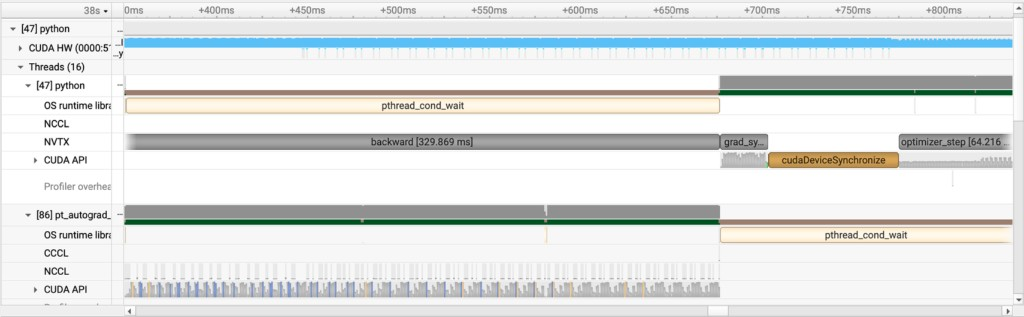
\includegraphics[width=\linewidth]{ddp_nonoverlap.png}
% 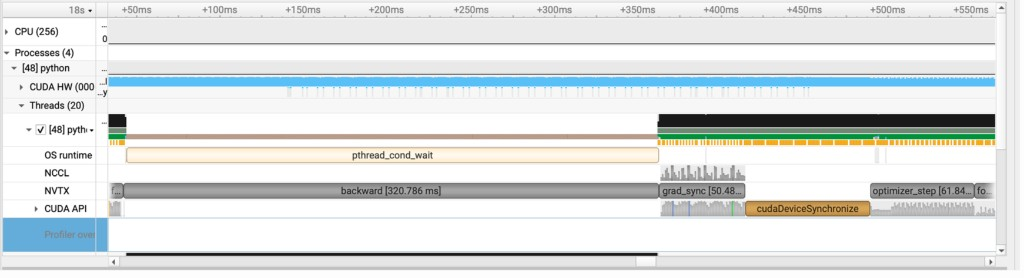
\includegraphics[width=\linewidth]{ddp_overlap.png}
\end{answer}


% =========================================================
\section{Optimizer State Sharding}
% =========================================================

\problem{optimizer\_state\_sharding}{15}
Implement a sharded-optimizer wrapper with \texttt{\_\_init\_\_(params, optimizer\_cls, **kwargs)}, \texttt{step}, and \texttt{add\_param\_group}; each rank keeps optimizer state for only its shard and syncs parameters after \texttt{step}.
\deliverable{Passes \texttt{uv run pytest tests/test\_sharded\_optimizer.py} reliably.}
\begin{answer}
\end{answer}


\problem{optimizer\_state\_sharding\_accounting}{5}

\subq{a} Peak memory with/without optimizer-state sharding (1 node, 2 GPUs, xl), measured after model init, before optimizer step, and after optimizer step. Break down memory by parameters / optimizer state / etc.
\deliverable{2--3 sentence response with peak memory and a breakdown.}
\begin{answer}
\end{answer}

\subq{b} Per-iteration time with and without optimizer-state sharding.
\deliverable{2--3 sentence response with your timings.}
\begin{answer}
\end{answer}

\subq{c} How does your implementation differ from ZeRO stage 1 ($P_{os}$)?
\deliverable{2--3 sentence summary focusing on memory and communication volume.}
\begin{answer}
\end{answer}


% =========================================================
\section{Fully-Sharded Data Parallel}
% =========================================================

\problem{fsdp}{15}
Implement an FSDP wrapper that shards \texttt{Linear}/\texttt{Embedding} weights, all-gathers in time for forward and backward, reduce-scatters gradients, frees gathered weights, supports optional \texttt{compute\_dtype}, and provides \texttt{finish\_gradient\_synchronization}.
\deliverable{Passes \texttt{uv run pytest tests/test\_fsdp.py} reliably (run multiple times).}
\begin{answer}
\end{answer}


\problem{fsdp\_accounting}{5}

\subq{a} Expected peak-memory savings for FSDP (ignoring preallocated all-gather buffers).
\deliverable{2--3 sentence response.}
\begin{answer}
\end{answer}

\subq{b} Profile xl on two GPUs: does the weight all-gather finish in time for the forward pass?
\deliverable{2--3 sentence response with Nsight screenshots.}
\begin{answer}
\end{answer}


% =========================================================
\section{Parallelism Analysis (Written)}
% =========================================================

\problem{alternate\_ring\_all\_reduce}{1}
For the alternate ring all-reduce algorithm given in the handout, how long does it take (egress bandwidth $W$, tensor size $S$, $N$ devices)?
\deliverable{Answer in terms of $S, N, W$, with one-sentence justification.}
\begin{answer}
\end{answer}


\problem{data\_parallel\_calcs}{3}
(FP16 weights/activations, ignore non-matmul FLOPs.)

\subq{a} Backward-pass FLOPs with $N_{\mathrm{DP}}$ data parallelism.
\deliverable{Answer in terms of $B, D, D_{\mathrm{FF}}, N_{\mathrm{DP}}$ with one-sentence justification.}
\begin{answer}
\end{answer}

\subq{b} Backward-pass communication time with $N_{\mathrm{DP}}$ data parallelism.
\deliverable{Answer in terms of subset of $B, D, D_{\mathrm{FF}}, N_{\mathrm{DP}}, W$ with one-sentence justification.}
\begin{answer}
\end{answer}

\subq{c} How large can $N_{\mathrm{DP}}$ grow before communication bottlenecks?
\deliverable{Inequality with $N_{\mathrm{DP}}$ on one side; right-hand side in terms of subset of $B, D, D_{\mathrm{FF}}, C, W$.}
\begin{answer}
\end{answer}


\problem{fsdp\_calcs}{3}

\subq{a} FLOPs for the forward and backward pass with $N_{\mathrm{FSDP}}$.
\deliverable{Two answers in terms of $B, D, D_{\mathrm{FF}}, N_{\mathrm{FSDP}}$ with two one-sentence justifications.}
\begin{answer}
\end{answer}

\subq{b} Communication time for the forward and backward pass with $N_{\mathrm{FSDP}}$.
\deliverable{Two answers in terms of a subset of $B, D, D_{\mathrm{FF}}, N_{\mathrm{FSDP}}, W$.}
\begin{answer}
\end{answer}

\subq{c} Scaling bounds for $N_{\mathrm{FSDP}}$ in forward and backward.
\deliverable{Two inequalities with $N_{\mathrm{FSDP}}$ on one side.}
\begin{answer}
\end{answer}


\problem{tp\_calcs}{4}

\subq{a} Backward pass of the TP strategy in the handout, in terms of $\mathbf{dy}$, sharded weights, saved activations, and communication primitives; produce $\mathbf{dW}_1^{(i)}, \mathbf{dW}_2^{(i)}, \mathbf{dW}_3^{(i)}$, and $\mathbf{dx}$.
\deliverable{A series of equations describing the TP backward pass.}
\begin{answer}
\begin{align*}
\mathbf{dy} &= \\
% ... fill in your derivation here.
\end{align*}
\end{answer}

\subq{b} Forward and backward FLOPs with $N_{\mathrm{TP}}$.
\deliverable{Two answers in terms of $B, D, D_{\mathrm{FF}}, N_{\mathrm{TP}}$.}
\begin{answer}
\end{answer}

\subq{c} Forward and backward communication time with $N_{\mathrm{TP}}$.
\deliverable{Two answers in terms of a subset of $B, D, D_{\mathrm{FF}}, N_{\mathrm{TP}}, W$.}
\begin{answer}
\end{answer}

\subq{d} Scaling bounds for $N_{\mathrm{TP}}$ in forward and backward.
\deliverable{Two inequalities with $N_{\mathrm{TP}}$ on one side.}
\begin{answer}
\end{answer}


\problem{fsdp\_tp\_calcs}{6}

\subq{a} Forward-pass FLOPs with $N_{\mathrm{FSDP}}$ FSDP + $N_{\mathrm{TP}}$ TP.
\deliverable{Answer in terms of $B, D, D_{\mathrm{FF}}, N_{\mathrm{FSDP}}, N_{\mathrm{TP}}$.}
\begin{answer}
\end{answer}

\subq{b} Forward-pass communication time assuming FSDP-axis and TP-axis collectives can be overlapped.
\deliverable{Answer in terms of a subset of $B, D, D_{\mathrm{FF}}, N_{\mathrm{FSDP}}, N_{\mathrm{TP}}, W$ (expected to be a max of two quantities).}
\begin{answer}
\end{answer}

\subq{c} With overlap, how large can $N = N_{\mathrm{TP}} N_{\mathrm{FSDP}}$ grow before the forward pass is communication bottlenecked? Find the optimal split.
\deliverable{Inequality with $N$ on one side, plus justification.}
\begin{answer}
\end{answer}

\subq{d} Same question but assuming no overlap between FSDP and TP collectives.
\deliverable{Inequality with $N$ on one side, plus justification.}
\begin{answer}
\end{answer}


% =========================================================
\section{Leaderboard (Optional)}
% =========================================================

\problem{leaderboard}{10}
Report your best wall-clock time for one full 8B training step on 2 B200 GPUs (bs 2, seq len 32768, BF16, causal).
\deliverable{Your best wall-clock time.}
\begin{answer}
\end{answer}


\end{document}
